% To generate a PDF from this document, run the following code in R:
%
%   Sweave("algorithms.Rnw")
%   tools::texi2pdf("algorithms.tex")
%
%
\documentclass[final]{siamart171218}
%\VignetteIndexEntry{Algorithms for NMF and topic modeling}
%\VignettePackage{fastTopics}
\usepackage{Sweave}
\usepackage{amsmath}
\usepackage{amssymb}
\usepackage{bm}
\setlength{\oddsidemargin}{0.65in}
\setlength{\evensidemargin}{0.65in}

\title{Algorithms for fitting topic models and non-negative matrix 
  factorizations to count data}
\author{Peter Carbonetto\thanks{Department of Human Genetics and the 
  Research Computing Center, University of Chicago, Chicago, IL}}

\begin{document}

\maketitle

\section{Introduction}
In this document, we study the problem of finding two non-negative
matrices, $F$ and $L$, minimizing the following loss function:
\begin{equation}
\ell(L,F) = 
-\sum_{i=1}^n \sum_{j=1}^m x_{ij} \log \lambda_{ij} + 
\sum_{i=1}^n \sum_{j=1}^m \lambda_{ij},
\label{eq:loss}
\end{equation}
where $\lambda_{ij} = \sum_{k=1}^K l_{ik} f_{jk}$, and $X$, $L$ and
$F$ are matrices of dimension $n \times m$, $n \times K$ and $m \times
K$, respectively, with non-negative entries $x_{ij}, l_{ik}, f_{jk}$.
(In the discussion and derivations below, $K$ is assumed to be 2 or
greater---the special case of $K = 1$, which has a relatively simple
solution, is treated in Appendix \ref{sec:rank1}.) Since \eqref{eq:loss}
is not convex when $K \geq 2$, we seek only to find a local minimum.

There are several ways to motivate minimizing \eqref{eq:loss}. One
motivation begins by modeling the counts $x_{ij}$ using the Poisson
distribution,
\begin{equation}
x_{ij} \sim \mathrm{Poisson}(\lambda_{ij}),
\label{eq:poisson}
\end{equation}
where $\mathrm{Poisson}(\lambda)$ denotes the Poisson distribution
with mean (and variance) $\lambda$. Next, by setting each of the
Poisson rates to be a simple linear combination, $\lambda_{ij} =
\sum_{k=1}^K l_{ik} f_{jk}$, the loss function \eqref{eq:loss} is
recovered as the negative log-likelihood of this model (with terms
that do not depend on either $F$ or $L$ omitted from the
expression). From this point-of-view, solving \eqref{eq:loss} is
equivalent to maximum-likelihood estimation (MLE) of $F$ and $L$ for
the Poisson model \eqref{eq:poisson}, and, hence, it is sometimes called
``Poisson non-negative matrix factorization.''

A second point-of-view provides additional intuition behind
\eqref{eq:loss}. This loss function can be also viewed as measuring
how well the low-rank factorization $LF^T$ approximates $X$; that is,
choices of $L$ and $F$ that achieve lower values of $\ell(L,F)$
reconstruct $X$ more accurately. The precise quality measure that
yields \eqref{eq:loss} is a Bregman divergence $D_{\phi}(X, LF^T)$
\cite{bregman-1967} with $\phi(x) = \sum_t x_t \log x_t$ as the choice
of generating convex function [refs]. To draw an analogy to other
matrix factorization methods such as principal components analysis
(PCA) or factor analysis \cite{engelhardt-stephens-2010}, we refer to
$L$ as the ``loadings'' matrix, and $F$ the ``factors'' matrix. (In
other papers, $L$ and $F$ are called the ``activations'' and ``basis
vectors,'' respectively).

Minizing \eqref{eq:loss} can also be motivated in a third way by
connecting it to fitting topic models [refs]---we elaborate on this
connection in the next section (``Connection to topic modeling'').

As you can probably gather by these three motivations, the problem of
minizing \eqref{eq:loss} is already very well-studied (e.g.,
[refs]). However, we have a particular focus on developing efficient
algorithms for count data sets that are large and sparse---by {\em
  sparse}, we mean that most of the counts $x_{ij}$ are zero. It
turns out that existing algorithms do not seem to accommodate large,
sparse data sets very well. Here we will look closely at the
computational properties of this optimization problem, and use these
investigations to help us design efficient algorithms for solving
\eqref{eq:loss} in the setting of large, sparse data sets.

To illustrate why this matters, consider computing the loss function
\eqref{eq:loss}. This is easy to implement in R:
\begin{Schunk}
\begin{Sinput}
> # Code goes here.
\end{Sinput}
\end{Schunk}

Also explain the difficulty of this optimization problem, and why this
motivates us to revisit algorithms for efficiently solving this
problem.  Despite the fact that this problem is well-studied, it turns
out, as we will see, that existing solutions are inadequate for large,
sparse data sets.



\section{Connection to topic modeling}
By optimizing \eqref{eq:loss} subject to the non-negativity
constraints, we are also optimizing a topic model [refs]. Here we make
this connection clear.

{\em Give R code here implementing this transformation.}

\section{An EM algorithm}
{\em Text goes here.}

\section{Evaluating convergence}
{\em Text goes here.}

\section{EM, revisited}
{\em Text goes here.}

In this example we embed parts of the examples from the
\texttt{kruskal.test} help page into a \LaTeX{} document:
\begin{Schunk}
\begin{Sinput}
> data(airquality, package = "datasets")
> library("stats")
> kruskal.test(Ozone ~ Month,data = airquality)
\end{Sinput}
\begin{Soutput}
	Kruskal-Wallis rank sum test

data:  Ozone by Month
Kruskal-Wallis chi-squared = 29, df = 4, p-value = 7e-06
\end{Soutput}
\end{Schunk}

which shows that the location parameter of the Ozone distribution
varies significantly from month to month. Finally, we include a
boxplot of the data, using
\begin{Schunk}
\begin{Sinput}
> boxplot(Ozone ~ Month, data = airquality)
\end{Sinput}
\end{Schunk}
\begin{center} 
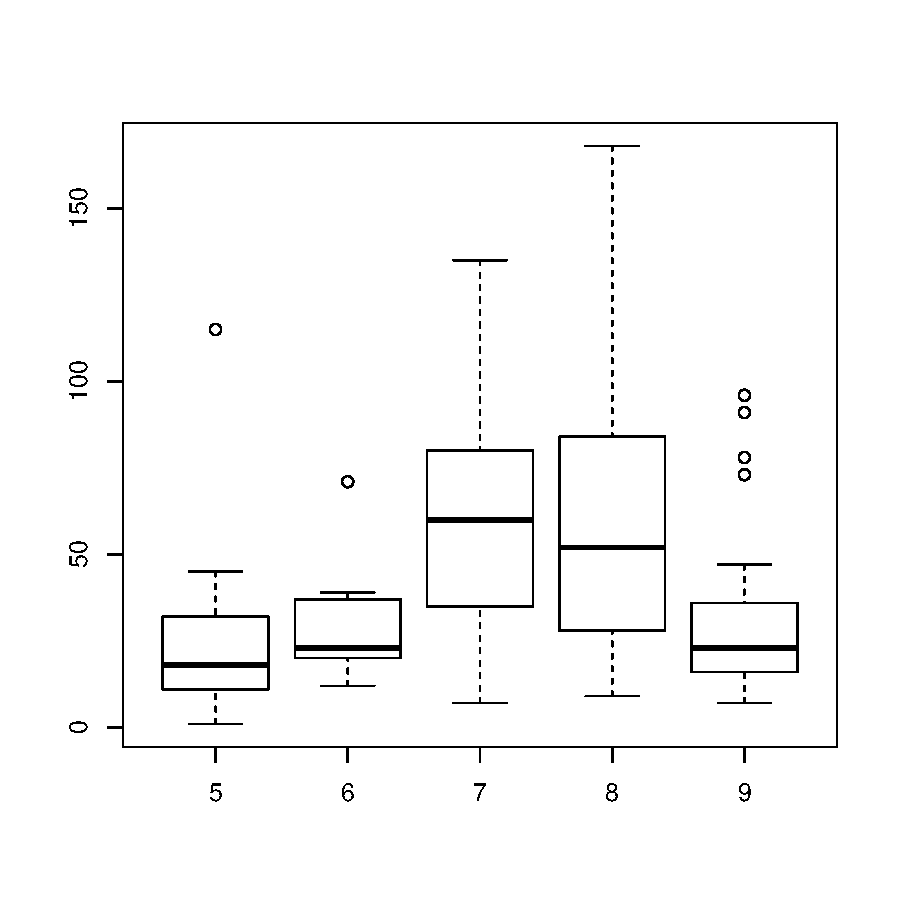
\includegraphics{algorithms-004}
\end{center}

Here is a citation: \cite{lee-2001}.

\subsection*{Acknowledgments}

Thanks to Youngseok Kim, Abhishek Sarkar, Jason Willwersheid, Zihao
Wang, Kushal Dey, Kevin Luo, Joyce Hsiao, Anthony Hung, Matthew
Stephens, and many other members of the Stephens lab, former and past,
for their valuable input. Also acknowledge the Research Computing
Center.

\appendix

\section{The rank-one case}
\label{sec:rank-1}
In the special case of $k = 1$, the Poisson rates can be expressed as
a simple outer product of two vectors,
\begin{equation*}
\Lambda = lf^T,  
\end{equation*}
where $l = (l_1, \ldots, l_n)^T$ and $f = (f_1, \ldots, f_m)^T$, and
the loss function \eqref{eq:loss} simplifies to
\begin{equation}
\ell(L,F) = -\sum_{i=1}^n \sum_{j=1}^m x_{ij} \log(l_if_j)
            + \sum_{i=1}^n \sum_{j=1}^m l_i f_j.
\label{eq:loss-rank-1}
\end{equation}
Any choice of $l, f$ that minimizes \eqref{eq:loss-rank-1} must therefore
be solution to the following system of equations:
\begin{align*}
f_j &= \frac{\sum_{i=1}^n x_{ij}}{\sum_{i=1}^n l_i}, 
       \quad j = 1,\ldots,m, \\
l_i &= \frac{\sum_{j=1}^m x_{ij}}{\sum_{j=1}^m f_j}, 
       \quad i = 1,\ldots,n.
\end{align*}
Since the solution is only defined up to a scaling factor, we enforce
the constraint that the mean of $f$ is the same as the mean of $l$,
yielding the following very simple solution:
\begin{align*}
f_j &= \frac{1}{n} \sum_{i=1}^n x_{ij},
       \quad j = 1,\ldots,m, \\
l_i &= \frac{1}{m} \sum_{j=1}^m x_{ij},
       \quad i = 1,\ldots,n.
\end{align*}
In other words, the MLE for the rank-one matrix factorization is
recovered as the row and column means of $X$.

\bibliographystyle{siamplain}
\bibliography{algorithms}

\end{document}
